\section{Potenzfunktionen}\index{Funktion!Potenzfunktionen}\index{Potenzfunktionen}
\sectuntertitel{Funktionen hoch drei!}

\subsection*{Lernziele}

\begin{itemize}
\item Definition Ganzzahlige Potenzfunktion
\item Graphische Darstellung
\end{itemize}
\newpage


\subsection{Einstieg}

%%%%%%%%%%%%%%%%%%%%%%%%%%%%%%%%%%%%%%%%%%%%%%%%%%%%%%%%%%%%%%%%%
\subsubsection{Beispiel: Rationale Funktion\GESO{ (optional)}}

Betrachten wir einmal die Funktion $f: y = 0.1x^3 + x^2 + 2x + 3 - x^{-1}$ \zB mit Geogebra (\texttt{www.geogebra.org}).

\bbwGraph{-10}{4}{-7}{8}{%
  \bbwFunc{0.1*\x*\x*\x + \x*\x + 2*\x + 3 -1/\x}{-8.5:-0.2}
  \bbwFunc{0.1*\x*\x*\x + \x*\x + 2*\x + 3 -1/\x}{0.1:1.5}
}%%


Polynomfunktionen und rationale Funktionen sind «\textit{weiche}» Funktionen, die jedoch \textbf{Asymptoten}\index{Asymptote} (hier bei $x=0$) aufweisen können.
Ebenso sind die Extremwerte (lokale Maxima und Minima)\TALS{ wie auch die Wendepunkte} charakteristische Stellen und oft Gegenstand der Untersuchung.
Wir beschränken uns \TALS{vorerst }auf Funktionen der Art $f: y=a\cdot{}x^z$
mit $z \in \mathbb{Z}\backslash\{0\}$\TRAINER{ $z=0$ ist eine
  Proportionalität und somit hier unspannend}.

\newpage
\subsubsection{\GESO{Beispiel}\TALS{Repetition}: Reinquadratische Funktion}\index{quadratische Funktion}\index{Funktion!quadratische}

\begin{definition}{Reinquadratische Funktion}{}
Die Funktion

$f: y = a\cdot{}x^2$

heißt \textbf{Parabel zweiter Ordnung} oder rein-quadratische Funktion.
\end{definition}

Zeichnen Sie den Graphen der Funktion $f: y= \frac16 x^2$:

\bbwGraph{-7}{7}{-1}{6.5}{%%
  \TRAINER{
    \bbwFunc{\x*\x/6}{-6:6}
  }
}%%


\begin{bbwFillInTabular}{|c|c||c|c|}\hline
  x & \,\,\,\,\,y\,\,\,\,\, & x & \,\,\,\,\,y\,\,\,\,\, \\\hline\hline
  $0$ & \TRAINER{$0$}               &        &    \\\hline
  $1$ & \TRAINER{$\frac16$}         &  $-1$  & \TRAINER{$\frac16$} \\\hline
  $2$ & \TRAINER{$\frac23$}         &  $-2$  & \TRAINER{$\frac23$} \\\hline
  $3$ & \TRAINER{$\frac32$}         &  $-3$  & \TRAINER{$\frac32$} \\\hline
  $4$ & \TRAINER{$\frac32$}         &  $-4$  & \TRAINER{$\frac83$} \\\hline
  $5$ & \TRAINER{$4.1\overline{6}$} &  $-5$  & \TRAINER{$4.1\overline{6}$} \\\hline
  $6$ & \TRAINER{$6$}               &  $-6$  & \TRAINER{$6$} \\\hline
\end{bbwFillInTabular} 



\TALS{\newpage}
\TALS{
\begin{bemerkung}{}{}
Eine allgemeine quadratische Funktion besitzt auch noch einen linearen ($bx$) und einen konstanten ($c$) Anteil. Die allgemeine quadratische Funktion hat die Form

$$f: y= ax^2 + bx + c$$
\end{bemerkung}
}%% END TALS

\TALS{Beispiele zu allgemeinen quadratischen Funktionen finden sie im
  Buch \cite{marthaler21alg} ab Seite 260 insb. im Bild zu Aufg. 4 auf
  Seite 273.}%% END TALS

\newpage
\subsection{Parabel}\index{Parabel}

\begin{definition}{Parabel}{definition_parabel}
  Ist $n\in \mathbb{N}_{\ge 2}$, so wird der Graph der Potenzfunktion
  $$x\mapsto a\cdot{}x^n$$
  \textbf{Parabel} $n$-ter Ordnung genannt.
\end{definition}


Zeichnen Sie $y = \frac{1}{16}x^4$ im Bereich $[-3; 3]$ indem Sie für jeden 0.5-er $x$-Wert das zugehörige $y$ berechnen:

\bbwGraph{-4}{4}{-1}{6.5}{%%
  \TRAINER{\bbwFunc{\x*\x*\x*\x/16}{-3:3}}
}%%

\begin{tabular}{|c|c||c|c|}\hline
  x & \,\,\,\,\,\,\,\,\,y\,\,\,\,\,\,\,\,\, & x & \,\,\,\,\,\,\,\,\,y\,\,\,\,\,\,\,\,\, \\\hline\hline
  $  0$ & \TRAINER{$0    $}          &          &                    \\\hline
  $0.5$ & \TRAINER{$0.004$}          &  $-0.5$  & \TRAINER{$0.004$} \\\hline
  $1  $ & \TRAINER{$0.063$}          &  $-1  $  & \TRAINER{$0.063$} \\\hline
  $1.5$ & \TRAINER{$0.316$}          &  $-1.5$  & \TRAINER{$0.316$} \\\hline
  $2  $ & \TRAINER{$1.000$}          &  $-2  $  & \TRAINER{$1.000$} \\\hline
  $2.5$ & \TRAINER{$2.441$}          &  $-2.5$  & \TRAINER{$2.441$} \\\hline
  $3  $ & \TRAINER{$5.063$}          &  $-3  $  & \TRAINER{$5.063$} \\\hline
\end{tabular} 

\TRAINER{Was fällt auf? Der Graph von $x^4$ ist um $0$ viel flacher
  als der Graph von $x^2$.}%% end Trainer

\TALS{%%
  \newpage
  \begin{bemerkung}{Potenzfunktion}{definition_potenzfunktion}
  Eine Funktion der Art
$$f: y=a\cdot{}x^r$$
  mit $r \in \mathbb{R}\backslash\{0\}$ heißt \textbf{Potenzfunktion}.
\end{bemerkung}

\begin{bemerkung}{Polynomfunktionen}{}
  Funktionen, deren Funktionsterm ein Polynom bilden werden
  \textbf{Polynomfunktionen} genannt:
  $$f: y=a_n\cdot{}x^n + a_{n-1}\cdot{}x^{n-1} + a_{n-2}\cdot{}x^{n-2} + ... + a_2\cdot{}x^2 + a_1 \cdot{} x + a_0 $$
\end{bemerkung}
%
}%% END TALS


\newpage
\subsection*{Aufgaben}
\aufgabenFarbe{Zeichnen Sie die Parabeln $$y=f(x) = x^n$$ für $n = 2$,
  $n=3$, $n=4$, $n=5$ und $n=6$ mit \texttt{geogebra.org}.
\\
Was fällt auf?}
%%\GESOAadBMTA{303ff}{1. (nur $n=3$ und $n=5$), 2. (nur $n=4$ und $n=6$)}

\TNTeop{}

\newpage

\subsubsection{Anwendung (optional)}
Boltzmannsches T-hoch-vier-Gesetz\index{Boltzmann!$T^4$-Gesetz}

\leserluft{}

Die Funktion $P(T) = \sigma\cdot\varepsilon\cdot
  A\cdot{}T^4$ beschreibt, welche Strahlungsleistung $P$ ein Körper der
  Oberfläche $A$ (in $ \text{m}^2$) bei Temperatur $T$ (in
  $\degre$Kelvin $= {}\degre\-\text{C}+273.15$) aussendet.

  $\sigma$ = Bolzmann Konstante = $5.6\cdot{}10^{-8}$
  
  $\varepsilon$ = Emissionswert

  \small{\texttt{(eg. https://ennologic.com/wp-content/uploads/2018/07/Ultimate-Emissivity-Table.pdf)}}

  \leserluft{}
  
  Rechenbeispiel:

\TNTeop{$T$ = 20 Grad Zimmertemperatur in Kelvin: 293.15;
  Brick (Haus) hat Emissionswert ca. 0.75; Haus Oberfläche $500 \text{m}^2$

  $$P(293.15) \approx 5.6\cdot{}10^{-8} \cdot{} 0.75 \cdot{} 500
  \cdot{} 293.15^4 \approx 155 \text{kW} $$
  Natürlich strahlt eine 20-grädige Umgebungstemperatur gleich viel
  wieder zurück, sodass keine 'Heizkosten' entstehen.

  Heizen wir das Haus nun zwei Grad wärmer, so erhalten wir:
  $$P(295.15) \approx 5.6\cdot{}10^{-8} \cdot{} 0.75 \cdot{} 500
  \cdot{} 295.15^4 \approx 159.4 \text{kW} $$

  Dies entspricht einer Differenz von 4.28 kW für nur zwei Grad wärmer
  im Haus!
  

}%% END TNT
\newpage

Zeichnen Sie des weiteren die Funktion $y = \frac{1}{9}x^3$:

\bbwGraph{-4}{4}{-5}{5}{%%
  \TRAINER{\bbwFunc{\x*\x*\x/9}{-3.5:3.5}}
}%%

\subsubsection{Symmetrien}\index{Symmetrien!von Parabeln}\index{Parabel!Symmetrie}
Was fällt für gerade und ungerade Exponenten auf? Gibt es Spiegelachsen
oder Spiegelpunkte?

\renewcommand{\mmPapier}[1]{\mmPapierZwei{#1}{16.4}}
\begin{tabular}{c|p{8cm}}
  $x^2$ & \vspace{0.1mm}\TNT{0.8}{An der $y$-Achse}\\\hline
  $x^3$ & \vspace{0.1mm}\TNT{0.8}{Am Ursprung $O(0|0)$}\\\hline
  $x^4$ & \vspace{0.1mm}\TNT{0.8}{wie $x^2$}\\\hline
  $x^5$ & \vspace{0.1mm}\TNT{0.8}{wie $x^3$}\\\hline
\end{tabular}
\renewcommand{\mmPapier}[1]{\mmPapierZwei{#1}{17.6}}


\GESO{Eine Zusammenfassung der wichtigsten Eigenschaften von
  Potenzfunktionen finden Sie im Buch \cite{marthaler21alg} Seite 296 oben.}
\newpage

\subsubsection{Referenzaufgabe}

Bestimmen Sie $a$ und $k$ so, dass der Graph von $y = a \cdot{} x^k$
durch die Punkte $P=\left(3 \middle| 1458\right)$ und
$Q=\left(-4\middle|8192\right)$ verläuft.

\TNT{15.2}{ Punkte einsetzen in die Funktionsgleichung:
  \gleichungZZ{1458}{a\cdot{}3^k}{8192}{a\cdot{}(-4)^k}
  Aus der oberen Gleichung das $a$ ermitteln ($a=\frac{1458}{3^k}$)
  (I) und in die zweite
  Gleichung einsetzen: $$8192 = \frac{1458}{3^k} \cdot{} (-4) ^k$$
  Exponent $k$ separieren:
  $$\frac{8192}{1458} = \left(\frac{-4}3\right)^k$$
  Problem: Logarithmen mit negativen Basen (hier $\frac{-4}3$)
  funktionieren nicht!
  
  Weil nun $k$ gerade sein muss, folgt dass $\left(\frac{-4}3\right)^k
  = \left(\frac43\right)^k$. Daraus ergibt sich
  $$\frac{8192}{1458} = \left(\frac{4}3\right)^k \Longrightarrow k =
  \log_{\frac43}\left(\frac{8192}{1458}\right) = 6$$
  Dieses $k$ nun in die Gleichung (I) einsetzen; dies
  liefert
  $$a=\frac{1458}{3^k} = 2.$$
}%% end TRAINER


\subsection*{Aufgaben}
\AadBMTA{305ff}{11. a) b) c), 13. a) c), (optional 17.,)  18.}
%%\TALSAadBMTA{197}{735. (6) (7) und (9) jeweils mit geogebra, 736. a) d),
%%  737. a) c), 739.}
\newpage


\subsection{Translationen}\index{Manipulation!Funktionen}\index{Funktions-Manipulation}\index{Translation!Funktion}
\sectuntertitel{Manipulation an Funktionsgraphen}
(Verschiebung\index{Verschiebung}, Spiegelung\index{Spiegelung},
Streckung\index{Streckung})

\TadBMTA{217}{13.3}
%%\TALSTadBFWA{163}{3}
Betrachten Sie die Funktionen

$$f(x) = a\cdot{}\left(\frac{x\TALS{-d}}b\right)^5\TALS{+c}$$
und
$$g(x) = a\cdot{}\left(\frac{x\TALS{-d}}b\right)^4\TALS{+c}$$

mit Geogebra (\texttt{geogebra.org})
und beschreiben Sie die Effekte der Parameter

$a$: \TRAINER{Streckung in $y$-Richtung. $a$ negativ: Spiegelung an der
$x$-Achse.}

\noTRAINER{\mmPapier{2.4}}

$b$: \TRAINER{Streckung entlang der $x$-Achse. $b$ negativ: Spiegelung
  an der $y$-Achse.}

\noTRAINER{\mmPapier{2.4}}

\TALS{%% nur TALS haben Verschiebungen
  $c$: \TRAINER{Verschiebung entlang der $y$-Achse}

\mmPapier{2.4}
}%% end TALS

\TALS{
$d$: \TRAINER{Verschiebung entlang der $x$-Achse (Verschiebung nach
  rechts verlangt ein negatives $d$.)}

\noTRAINER{  \mmPapier{2.4}}
}%% END TALS

\newpage

\subsubsection{Zusammenfassung der Translationen}


Wir betrachten die verschiedenen geometrischen
Funktions-«Manipulationen» (Abbildungen) am Beispiel {\color{red}$y =f(x) = \frac18 x^3$}.


\newcommand{\graphTranslationMultiColumn}[5]{%
  \multicolumn{3}{|l|}{#1}\\%%
\hline%%
\graphTranslationMultiColumnZ{#2}{#3}{#4}{#5}
}%% end new command \graphTranslationMultiColumn

\newcommand{\graphTranslationMultiColumnZ}[4]{%
\multirow{5}{6cm}{#1} &  & \multirow{2}{*}{\begin{minipage}{.3\textwidth}\raisebox{-8cm}{\includegraphics[width=\linewidth,height=60mm]{allg/funktionen/img/translation/#4}}\end{minipage}}\\[55mm]%%
&\fbox{#2}&\\%%
&&\\%%
&{\color{red}\fbox{#3}}&\\%%
&&\\%%
\hline%%
}%% end new command \graphTranslationMultiColumnZ

\TALS{%% Nur TALS haben Verschiebungen
\begin{tabular}{|p{7cm}|c|c|}%%
\hline%%
\graphTranslationMultiColumn{Verschiebung in $y$-Richtung...}{... um \textbf{zwei} Einheiten nach \textbf{oben}:}{$g(x)=f(x)\textbf{+2}$}{$g(x)=\frac18x^3\textbf{+2}$}{typ1.png}
\graphTranslationMultiColumnZ{... um \textbf{eine} Einheiten nach \textbf{unten}:}{$g(x)=f(x)\textbf{-1}$}{$g(x)=\frac18x^3\textbf{-1}$}{typ2.png}
\end{tabular}%%
}%% end TALS

\begin{tabular}{|p{7cm}|c|c|}%%
\hline%%
\graphTranslationMultiColumn{Spiegelung...}{... an der $x$-Achse:}{$g(x)=-f(x)$}{$g(x)=-\frac18x^3$}{typ3.png}
\graphTranslationMultiColumnZ{... an der $y$-Achse:}{$g(x)=f(-x)$}{$g(x)=\frac18(-x)^3$}{typ4.png}
\end{tabular}%%

\begin{tabular}{|p{7cm}|c|c|}%%
\hline%%
\graphTranslationMultiColumn{Streckung...}{... in $y$-Richtung (von der $x$-Achse aus) um Faktor \textbf{zwei}:}{$g(x)=\textbf{2}\cdot{}f(x)$}{$g(x)=\textbf{2}\cdot{}\frac18x^3$}{typ5.png}
\graphTranslationMultiColumnZ{... in $x$-Richtung (von der $y$-Achse aus) um Faktor \textbf{zwei}:}{$g(x)=f(\frac{1}{\textbf{2}}\cdot{}x)$}{$g(x)=\frac18(\frac{1}{\textbf{2}}\cdot{}x)^3$}{typ6.png}
\end{tabular}%%

\TALS{%% Nur TALS verschieben in x-Richtung
\begin{tabular}{|p{7cm}|c|c|}%%
\hline%%
\graphTranslationMultiColumn{Verschiebung in $x$-Richtung\footnote{Kein prüfungsrelevantes Thema.}...}{... um \textbf{zwei} Einheiten nach \textbf{links}:}{$g(x)=f(x\textbf{+2})$}{$g(x)=\frac18(x\textbf{+2})^3$}{typ7.png}
\graphTranslationMultiColumnZ{... um \textbf{zwei} Einheiten nach \textbf{rechts}:}{$g(x)=f(x\textbf{-2})$}{$g(x)=\frac18(x\textbf{-2})^3$}{typ8.png}
\end{tabular}%%
}%% END TALS
\newpage

\subsection*{Aufgaben}
\GESO{
Skizzieren Sie $-\frac{1}{2}x^3 - 1$ im Bereich $x$ = -2 bis $x$ = +2.

\bbwGraph{-4}{4}{-5}{3}{%%
  \TRAINER{%
    \bbwFunc{-0.5*\x*\x*\x-1}{-2:2}%
  }%%
}%

Vergleichen Sie die neue Funktion mit der Parabel $y=x^3$.

\TNT{5.2}{Die neue Funktion ist an der $y$-Achse gespiegelt, ist um
  50\% gestaucht ($y$-Richtung) und ist um eine Einheit nach unten
  ($x$-Richtung) verschoben worden.}
}%% END GESO

\AadBMTA{304ff}{9. a) d) e)., 5 a) c) d) e)}

\TALS{
  \aufgabenFarbe{Zeichnen Sie mit \texttt{geogebra.org} die Funktion
    $f(x) = \frac1{10}(x^3 - 3x^2 + 3)$
    \\
    Definieren Sie anschließend die Funktion $$g(x) = a\cdot{}f((x+s)\cdot{}b)+r.$$
\\
    Entscheiden Sie, welche Veränderungen die Parameter $a$, $b$, $r$
    und $s$ bewirken.\\
    Starten Sie mit $a=1$, $b=1$, $r=0$ und $s=0$.
  }%% END Aufgabenfarbe
  \TNT{4}{
    $r$: Verschiebung nach oben\\
    $s$: Verschiebung nach links\\
    $a$: Streckung in $y$-Richtung\\
    $b$: Stauchung in $x$-Richtung
  }%% END TNT
}%% END TALS



%%  OLAT Arbeitsblatt
\GESO{\olatLinkArbeitsblatt{Positive Potenzfunktionen zuordnen}{https://olat.bms-w.ch/auth/RepositoryEntry/6029794/CourseNode/104752086007823}{(alle Beispiele)}}%% END olatLinkArbeitsblatt
\TALS{\olatLinkArbeitsblatt{Positive Potenzfunktionen zuordnen}{https://olat.bms-w.ch/auth/RepositoryEntry/6029786/CourseNode/105597875231723}{(alle Beispiele)}}%% END olatLinkArbeitsblatt


\olatLinkTALSStrukturaufgabenSPF{Teil 2}{15ff}{48. und 51.}
%%\TALS{\aufgabenFarbe{Strukturaufgaben SPF Teil 2: Taschenrechner: S. 15ff:  Aufg. 48. und 51.}%% END Aufgabenfarbe
%%}%% END TALS

%%\TALSAadBMTA{197 ff.}{739., 743. c), 745. c), 738.*}

\olatLinkGESOKompendium{3.3.1.}{26}{28., 29.}
\newpage



%%%%%%%%%%%%%%%%%%%%%%%%%%%%%%%%%%%%%%%%%%%%%%%%%%%%%%%%%%%%%%%%%%%%%%%%%%%%%%%%%%%
\subsection{Hyperbel}\index{Hyperbel (negative Exponenten)}

(«Hyperbel» Griechisch = «über das Ziel hinaus werfen»)


Zur Erinnerung:
\begin{multicols}{2}
\begin{itemize}
	\item $x^{-1} = \frac{1}{x}$
	\item $x^{-2} = \frac{1}{x^2}$
	\item $x^{-3} = \frac{1}{x^3}$
	\item $x^{-4} = \frac{1}{x^4}$
	\item $x^{-5} = \frac{1}{x^5}$
  \item ...
\end{itemize}
\end{multicols}

Zeichnen Sie die Funktion $f: y = x^{-1}$ im Definitinosbereich
$\DefinitionsMenge{} = [-5;5]\TRAINER{\backslash \{0\}}\noTRAINER{......}$

\bbwGraph{-6}{6}{-3}{3}{%%
  \TRAINER{\bbwFunc{1/\x}{-5:-0.3}}
  \TRAINER{\bbwFunc{1/\x}{0.3:5}}

}%%

\newpage


Zeichnen Sie zusätzlich Funktion $f: y = x^{-2}$ im Definitionsbereich $[-5;5]$:

\bbwGraph{-6}{6}{-5}{5}{%%
  % x^-2
  \TRAINER{\bbwFuncC{1/(\x * \x)}{-5:-0.447}{green}}%% 0.447 = 1/sqrt (5)
  \TRAINER{\bbwFuncC{1/(\x * \x)}{0.447:5}{green}}
  \TRAINER{\bbwLetter{2.5,0.5}{x^{-2}}{green}}
  \TRAINER{\bbwLetter{-1.5,1}{x^{-2}}{green}}

  %x^-3
%  \TRAINER{\bbwFuncC{1/(\x * \x * \x)}{-5:-0.584}{blue}}
%  \TRAINER{\bbwFuncC{1/(\x * \x * \x)}{0.584:5}{blue}}
%  \TRAINER{\bbwLetter{0.8,0.3}{x^{-3}}{blue}}
%  \TRAINER{\bbwLetter{-1.2,-3.8}{x^{-3}}{blue}}
%  \TRAINER{\bbwLetter{1.2,4.5}{x^{-3}}{blue}}

}%%

\begin{definition}{Hyperbel}{definition_hyperbel}
  Der Graph einer Potenzfunktion $$f: y=ax^z$$
  mit $z \in \{-1, -2, -3, -4, ...\}$ heißt
\textbf{Hyperbel}\index{Hyperbel} der Ordnung $z$.
\end{definition}

Der Definitionsbereich von Hyperbeln entspricht dem Definitionsbereich
des Funktionsterms. Merke: Es darf nicht durch Null geteilt werden:

$$x^{-5} = \frac{1}{x^5} \Longrightarrow \DefinitionsMenge{} = \mathbb{R} \backslash \{0\}$$


\subsection*{Aufgaben}
\AadBMTA{306ff}{19. Zeichnung mit geogebra.org, 20.
  Zeichnung mit geogebra.org}
%%\TALSAadBMTA{205}{771. a) c) d) e) g) h) j)}


\newpage

\subsubsection{Charakteristiken}
\textbf{Spiegelungen:}\\

Welche Funktionen $x$, $x^{-1}$, $x^{-2}$, $x^{-3}$ sind an welchen Achsen bzw. Punkten gespiegelt?

\renewcommand{\mmPapier}[1]{\mmPapierZwei{#1}{16.0}}
\begin{tabular}{c|p{10cm}}
  $x^{-1}$ &  \TNT{0.8}{Am Ursprung $O(0|0)$ : Punktspiegelung}\\
  \hline
  $x^{-2}$ &  \TNT{0.8}{An der $y$-Achse: Achsensymmetrie}\\
  \hline
  $x^{-3}$ &  \TNT{0.8}{Am Ursprung $O(0|0)$: Punktspiegelung}\\
  \hline
  $x^{-4}$ &  \TNT{0.8}{An der $y$-Achse: Achsensymmetrie}\\
  \hline  
\end{tabular}
\renewcommand{\mmPapier}[1]{\mmPapierZwei{#1}{17.6}}


\paragraph{Definitions- und Wertebereiche:}

Geben Sie für die obigen Funktionen an, was ihr Definitions- bzw. Wertebereich ist\footnote{Grundmenge ist $\mathbb{R}$.}:

\begin{tabular}{c|c|c}
Funktionsterm & Definitionsbereich $\DefinitionsMenge{}$& Wertebereich $\Wertebereich{}$\\ \hline
  $x^{-1}$ & \TRAINER{$\mathbb{R}\backslash\{0\}$} &  \TRAINER{$\mathbb{R}\backslash\{0\}$}\\ \hline
  $x^{-2}$ & \TRAINER{$\mathbb{R}\backslash\{0\}$} &  \TRAINER{$\mathbb{R}^{+}\backslash\{0\}$}\\ \hline
  $x^{-3}$ & \TRAINER{$\mathbb{R}\backslash\{0\}$} &  \TRAINER{$\mathbb{R}\backslash\{0\}$}\\ \hline
  $x^{-4}$ & \TRAINER{$\mathbb{R}\backslash\{0\}$} &  \TRAINER{$\mathbb{R}^{+}\backslash\{0\}$}\\ \hline
\end{tabular}


\GESO{\subsection*{Aufgaben}}
\olatLinkGESOKompendium{3.3}{26}{28. bis 31.}
\GESO{\aufgabenFarbe{Aufgabe der Nullserie 2 (zweite Nullserie): Aufg. 7 auf Seite 3}}
\GESO{\aufgabenFarbe{Maturaprüfung 2016, Aufg. 8 (Graphen zuordnen)}}

\newpage

\newpage

%%%%%%%%%%%%%%%%%%%%%%%%%%%%%%%%%%%%%%%%%%%%%%%%%%%%%%%%%%%%%%%%%%%%%%%%%%%%%%%%%%%

\subsection{Zusammenfassungen und Überblick}\index{Potenzfunktionen!Überblick}

$$y = a\cdot{}x^z$$

$z$ gerade: Gespiegelt an der $y$-Achse

$z$ ungerade: Gespiegelt am Ursprung $O=(0|0)$

Ist ${\color{ForestGreen}a>0}$\TRAINER{ (grün in der Graphik)}, so sind Graphen mit
geraden Exponenten nach oben geöffnet bzw. mit ungeraden Exponenten im
Quadranten I und III.

Ist ${\color{red}a<0}$\TRAINER{ (rot/orange in der Graphik)}, so sind Graphen mit
geraden Exponenten nach unten geöffnet bzw. mit ungeraden Exponenten
im Quadranten II und IV.


\TRAINER{%
  \includegraphics[width=8.5cm]{allg/funktionen/img/potenzfct/potenzFunktionenGerade.png}\hfill{}\includegraphics[width=8.5cm]{allg/funktionen/img/potenzfct/potenzFunktionenUngerade.png}
}%% END Trainer
\noTRAINER{%
  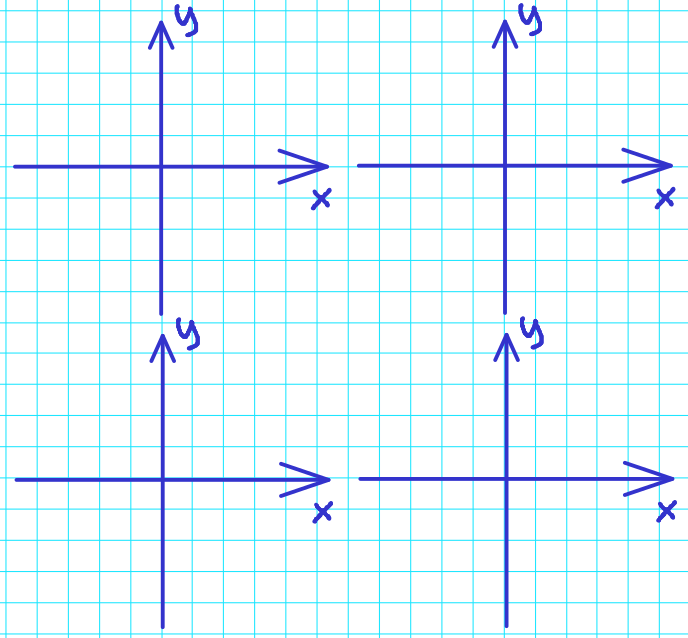
\includegraphics[width=8.5cm]{allg/funktionen/img/potenzfct/potenzFunktionenLeer.png}\hfill{}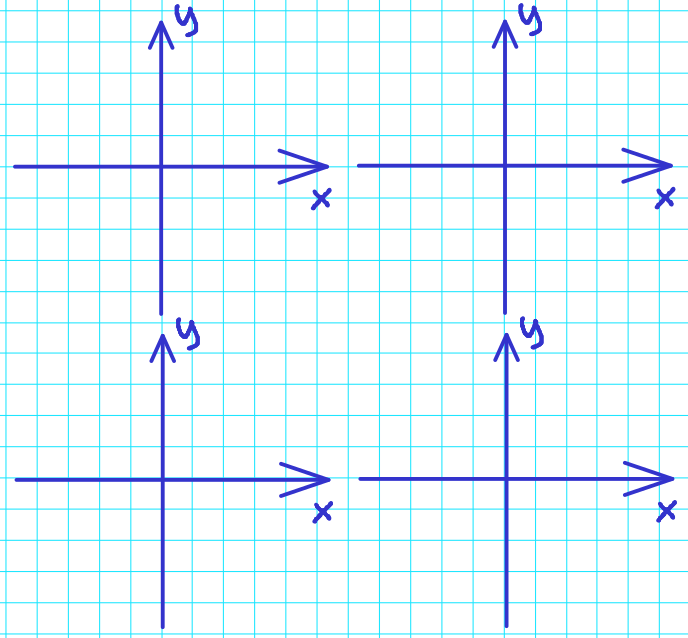
\includegraphics[width=8.5cm]{allg/funktionen/img/potenzfct/potenzFunktionenLeer.png}
}%% END Trainer


\subsection*{Aufgaben}
\AadBMTA{307}{25. b) c), 26. a)\TALS{ b)}, 27. b) c)\TALS{, 33*}}

\newpage


\newpage
